\section{A joint transition for reflected log-gamma moments}
\label{moment:sec}

The reflected family already considered in the manuscript is
\begin{equation}\label{moment:def}
 M_{n,m}=\int_0^1 f(x)^n f(1-x)^m\,dx,
 \qquad f(x)=\log\Gamma(x),\quad n,m\in\mathbb Z_{\ge0}.
\end{equation}
These mixed moments occur in Amdeberhan et al.~\cite[Section 5]{Amdeberhan2011}.
The manuscript proves that, for each fixed $m$,
\begin{equation}\label{moment:fixed}
 M_{n,m}\sim \frac{\gamma^m n!}{(m+1)^{n+1}},\qquad n\longrightarrow\infty,
\end{equation}
and develops the associated residues, late coefficients, and optimal truncation.
Its reflected-moment section explicitly leaves uniformity for growing $m$ open.
The result below identifies a transition where the leading expression
\eqref{moment:fixed} acquires a nontrivial factor. It concerns simultaneous
growth of the two exponents, rather than the late truncation index in the
already established fixed-$m$ expansion.

\subsection{The critical scale and the first correction}
Write $\gamma$ for Euler's constant, and define
\begin{equation}\label{moment:constants}
 c=\frac{\zeta(2)}{2\gamma}-\gamma,
 \qquad d=\frac{\zeta(3)}{3\gamma}
              -\frac{\zeta(2)^2}{8\gamma^2}.
\end{equation}
The constant $c$ is positive; for example $0<\gamma<0.6$ and
$\zeta(2)>1$ suffice to prove this. Its numerical value is
$c=0.8476712247576688767895678092\ldots$.
For $m\ge1$ put
\begin{equation}\label{moment:parameters}
 t=\frac{n}{m+1},\qquad \lambda=me^{-t},\qquad
 \mathcal R_{n,m}=\frac{(m+1)^{n+1}M_{n,m}}{\gamma^m n!}.
\end{equation}
All limits below are along integer pairs $(n,m)$ satisfying the stated
conditions. In particular $n>0$ and $t\ge2$ for all sufficiently large $m$.

\begin{theorem}[Uniform reflected-moment transition]\label{moment:thm:transition}
Fix $S>0$. Uniformly as $m\to\infty$ in the strip
$|t-\log m|\le S$, one has
\begin{equation}\label{moment:transition}
 \boxed{\displaystyle
 \mathcal R_{n,m}=e^{c\lambda}
 \left(1+\frac{C_1(t,\lambda)}m
              +O_S\!\left(\frac{t^2}{m^2}\right)\right),}
\end{equation}
where the correction is the explicit polynomial
\begin{equation}\label{moment:C1}
 C_1(t,\lambda)
 =\lambda\left[c\left(\frac t2-1\right)-2\gamma\right]
  +\lambda^2\left[\frac{c^2t}{2}+\gamma^2+d\right].
\end{equation}
Consequently, if $n/(m+1)-\log m\to s\in\mathbb R$, then
\begin{equation}\label{moment:profile}
 \mathcal R_{n,m}\longrightarrow \exp\!\left(c e^{-s}\right).
\end{equation}
\end{theorem}

For example, choosing $n$ to be the nearest integer to $(m+1)\log m$
gives $\mathcal R_{n,m}\to e^c=2.3342\ldots$, rather than $1$.
Thus the fixed-reflected-exponent leading term cannot be used uniformly
through this transition. The exact exponential in \eqref{moment:profile}
is more informative than a first-order correction to a fixed-$m$ formula.

\subsection{The exact probability representation}
Set
\[
 B(x)=\log\Gamma(1-x),\qquad \ell(x)=\log\Gamma(1+x).
\]
The standard expansions needed below are convergent for $|x|<1$
\cite[Section 5.7]{DLMF}:
\begin{align}\label{moment:endpoint-series}
 \ell(x)&=-\gamma x+\frac{\zeta(2)}2x^2
                    -\frac{\zeta(3)}3x^3+\cdots,\notag\\
 B(x)&=\gamma x+\frac{\zeta(2)}2x^2
                    +\frac{\zeta(3)}3x^3+\cdots.
\end{align}
The inequality $\psi'(x)>0$, together with $\psi(1)=-\gamma<0$,
shows that $f(x)>0$ on $(0,1)$. Log-convexity of $\Gamma$ between $1$
and $2$ gives $\ell(x)\le0$, hence
\begin{equation}\label{moment:elementary-bound}
 0<f(x)\le-\log x\quad(0<x<1),\qquad
 \int_0^1 f(x)^m\,dx\le m!.
\end{equation}

Let $r=m+1$ and let $Y$ have the gamma density with shape $n+1$ and rate $r$:
\[
 p(y)=\frac{r^{n+1}}{n!}y^n e^{-ry},\qquad y>0.
\]
Its mode is exactly $t=n/r$. The substitution $x=e^{-y}$ in
\eqref{moment:def} gives the identity
\begin{equation}\label{moment:expectation}
 \mathcal R_{n,m}=\mathbb E\,e^{E_m(Y)},
\end{equation}
where
\begin{equation}\label{moment:weight}
 E_m(y)=n\log\left(1+\frac{\ell(e^{-y})}{y}\right)
       +m\log\left(\frac{B(e^{-y})}{\gamma e^{-y}}\right).
\end{equation}
The expressions inside both logarithms are positive for $y>0$.
Equation \eqref{moment:expectation} is exact, with no asymptotic interchange.

\subsection{Why the weighted tails are negligible}
Ordinary gamma concentration is not by itself sufficient in
\eqref{moment:expectation}: the multiplying weight can grow on the left.
We therefore prove the required estimate explicitly.

\begin{lemma}[Uniform weighted localization]\label{moment:lem:localization}
For each fixed $S>0$, there are positive constants $C_S,c_S$ such that,
for all sufficiently large $m$ with $|t-\log m|\le S$,
\begin{equation}\label{moment:localization}
 \mathbb E\left[e^{E_m(Y)}\mathbf1_{\{|Y-t|>1\}}\right]
 \le C_S\exp\!\left(-c_S\frac m t\right).
\end{equation}
Unweighted tails with any fixed polynomial factor in $|Y-t|$ obey the
same type of bound, after altering the constants.
\end{lemma}

\begin{proof}
Let $y_0=\log2$. For $0<x\le1/2$, positivity of the coefficients of $B$
and $\zeta(j)/j\le\zeta(2)/2$ for $j\ge2$ give
\[
 \frac{B(x)}{\gamma x}
 \le1+\frac{\zeta(2)x}{2\gamma(1-x)}
 \le1+C x,\qquad C=\frac{\zeta(2)}\gamma.
\]
Since $\ell\le0$, this implies
\begin{equation}\label{moment:weight-bound}
 e^{E_m(y)}\le \exp(Cme^{-y}),\qquad y\ge y_0.
\end{equation}

On $0<y<y_0$, use the original moment integral and
\eqref{moment:elementary-bound}. The unnormalized contribution is at most
$y_0^n m!$. Stirling's bounds show that the logarithm of its normalized
contribution is
\[
 -n\log t+O_S(n+m\log m).
\]
In the strip, $m\log m=O_S(n)$, so this is at most
$-\tfrac12n\log t$ for sufficiently large $m$.

On $y_0\le y\le t/2$, the weight is at most $e^{Cm/2}$.
The gamma lower-tail bound at half the mode is $e^{-c_0n}$ for a fixed
$c_0>0$ once $n$ is large. This follows directly from the moment-generating
function $(1-u/r)^{-n-1}$ and exponential Markov inequality.
Since $n/m\sim\log m$, the weighted contribution is $O(e^{-c_1mt})$.

On $t/2\le y\le t-1$, write $u=t-y$. The exact ratio to the density at
the mode satisfies
\begin{equation}\label{moment:density-ratio}
 \frac{p(t-u)}{p(t)}
 =\exp\{n\log(1-u/t)+ru\}
 \le\exp\!\left(-\frac{ru^2}{2t}\right).
\end{equation}
The weight in \eqref{moment:weight-bound} is at most $\exp(C\lambda e^u)$.
For $1\le u\le t/2$, the maximum of $e^u/u^2$ occurs at an endpoint.
As $\lambda\in[e^{-S},e^S]$ and $t=\log m+O_S(1)$, it follows that
\[
 C\lambda e^u\le \frac{ru^2}{4t}
\]
uniformly on this interval when $m$ is large. Multiplication by
\eqref{moment:density-ratio}, followed by integration and
$p(t)=O(\sqrt{r/t})$, gives $O_S(e^{-c_2m/t})$.

Finally, on $y\ge t+1$, the weight is bounded by $\exp(C\lambda/e)$.
The gamma upper-tail bound for a displacement of one from the mode is
$O_S(e^{-c_3m/t})$. For completeness, with mean $(n+1)/r=t+1/r$,
the usual gamma exponent at $t+1$ is
$(n+1)(\delta-\log(1+\delta))$, where
$\delta=(r-1)/(n+1)\asymp1/t$; this exponent is bounded below by a
positive constant times $r/t$.
The four estimates prove \eqref{moment:localization}. Inserting a fixed
polynomial in the tails only introduces polynomial factors, which can
be absorbed by reducing the positive exponential constant. The density
ratio or the same exponential Markov argument gives this last assertion.
\end{proof}

\subsection{Proof of the transition and its explicit correction}
\begin{proof}[Proof of Theorem~\ref{moment:thm:transition}]
For the calculation abbreviate
\[
 a=-\gamma,\quad a_2=\zeta(2)/2,\quad b=\zeta(2)/(2\gamma),
 \quad c=a+b.
\]
Let $V=Y-t$. Uniformly for $|v|\le1$, set
$x=(\lambda/m)e^{-v}$ and use \eqref{moment:endpoint-series} with its
analytic remainder. One obtains
\begin{equation}\label{moment:local-expansion}
 E_m(t+v)=A(v)+\frac{B_1(v)}m+O_S(m^{-2}),
\end{equation}
where
\begin{align}\label{moment:local-functions}
 A(v)&=\lambda e^{-v}\left(b+\frac{at}{t+v}\right),\notag\\
 B_1(v)&=\frac{a\lambda te^{-v}}{t+v}
 +\lambda^2e^{-2v}\left(d+\frac{a_2t}{t+v}
                            -\frac{a^2t}{2(t+v)^2}\right).
\end{align}
All derivatives of each fixed order used below are uniformly bounded
in this interval; $t/(t+v)$ is bounded once $t\ge2$.

The exact moments about the mode, rather than about the mean, are
\begin{align}\label{moment:central-moments}
 \mathbb EV&=r^{-1},&
 \mathbb EV^2&=t/r+2/r^2,\notag\\
 \mathbb EV^3&=5t/r^2+6/r^3,&
 \mathbb EV^4&=3t^2/r^2+26t/r^3+24/r^4.
\end{align}
They follow either from gamma raw moments or from
$\mathbb Ee^{zV}=e^{-tz}(1-z/r)^{-rt-1}$.
Taylor expand $e^{A(v)}$ through degree three and bound its fourth
remainder with \eqref{moment:central-moments}. The cubic term is
$O_S(t/m^2)$ because its signed moment, not its absolute third moment,
is used. Expand $e^{A(v)}B_1(v)$ through degree one with a quadratic
remainder. Lemma~\ref{moment:lem:localization} allows us to use full
gamma moments and discard the outer tails. The result is
\begin{align}\label{moment:first-reduction}
 e^{-A(0)}\mathcal R_{n,m}
 =1+\frac1m\left[B_1(0)+A'(0)
       +\frac t2\{A''(0)+A'(0)^2\}\right]
 +O_S(t^2/m^2).
\end{align}
Here replacing $r^{-1}$ by $m^{-1}$ changes only the stated remainder.

The local values are
\begin{align*}
 A(0)&=c\lambda,& A'(0)&=-\lambda(c+a/t),\\
 A''(0)&=\lambda(c+2a/t+2a/t^2),&
 B_1(0)&=a\lambda+\lambda^2(d+a_2-a^2/(2t)).
\end{align*}
Substitution into \eqref{moment:first-reduction} cancels all negative
powers of $t$ and yields
\[
 \lambda\{c(t/2-1)+2a\}
 +\lambda^2\{c^2t/2+ca+d+a_2\}.
\]
The relation $ca+a_2=\gamma^2$ gives \eqref{moment:C1}.
Since $t/m\to0$, the limit \eqref{moment:profile} follows immediately.
\end{proof}

\subsection{All fixed asymptotic orders}
\begin{theorem}[Constructive expansion to every fixed order]
\label{moment:thm:all-orders}
For each integer $J\ge0$, there are explicitly computable functions
$C_j(t,\lambda)$, polynomial in $\lambda$ and rational in $t$, such that
$C_0=1$, $C_1$ is \eqref{moment:C1}, and
\begin{equation}\label{moment:all-orders}
 \mathcal R_{n,m}=e^{c\lambda}
 \left[\sum_{j=0}^J\frac{C_j(t,\lambda)}{m^j}
 +O_{S,J}\!\left(\frac{t^{J+1}}{m^{J+1}}\right)\right]
\end{equation}
uniformly in $|t-\log m|\le S$. For each fixed $j$,
$C_j(t,\lambda)=O_{S,j}(t^j)$. The theorem asserts an expansion at every
fixed order, without asserting convergence of the infinite expansion.
\end{theorem}

The following finite differential prescription makes ``computable''
precise. Let $\epsilon$ be a formal variable and put
$r=(1+\epsilon)/\epsilon$. Define
\begin{align}\label{moment:formal-Phi}
 \Phi_\epsilon(v)=\epsilon^{-1}\Bigg[
 &(1+\epsilon)t\log\left(1+
 \frac{\ell(\lambda\epsilon e^{-v})}{t+v}\right)\notag\\
 &+\log\left(\frac{B(\lambda\epsilon e^{-v})}
                        {\gamma\lambda\epsilon e^{-v}}\right)\Bigg],\\
 K_\epsilon(z)&=\frac zr+
 \sum_{k\ge2}\left(\frac{t}{kr^{k-1}}+
                         \frac1{kr^k}\right)z^k.
 \label{moment:formal-K}
\end{align}
The quotient involving $B$ has constant term one, and both terms in
brackets vanish at $\epsilon=0$, so the formal expression is well defined.
With derivatives acting on $v$, the coefficients are
\begin{equation}\label{moment:coefficient-algorithm}
 C_j(t,\lambda)=e^{-c\lambda}[\epsilon^j]
 \left.\exp\!\bigl(K_\epsilon(\partial_v)\bigr)
                      e^{\Phi_\epsilon(v)}\right|_{v=0}.
\end{equation}
Only finitely many derivatives occur at a fixed order: the maximum
derivative order at $\epsilon^j$ is $2j$.

\begin{proof}[Proof of Theorem~\ref{moment:thm:all-orders}]
Expand \eqref{moment:weight} through order $J$ in $1/m$ on $|v|\le1$.
The convergent endpoint series make its remainder, together with any
fixed number of $v$ derivatives, uniformly $O_{S,J}(m^{-J-1})$.
Expand the resulting analytic amplitudes in $v$ through degree $2J+1$.
Gamma moment--cumulant identities give
\[
 \mathbb E|V|^{2J+2}=O_J\!\left((t/m)^{J+1}\right),
\]
while signed odd moments occur at integer powers of $1/m$ and have the
corresponding smaller order. These facts follow directly by expanding
the exact logarithm of the moment-generating function, which is
\eqref{moment:formal-K}. Lemma~\ref{moment:lem:localization} controls
the tails, including every polynomial moment used here.
Taylor's theorem therefore gives \eqref{moment:all-orders} with the
displayed remainder.

At each fixed order all derivatives at $v=0$ of
$t/(t+v)$ are rational functions of $t$, and all endpoint coefficients
are finite combinations of $\gamma$ and zeta values. The common
exponential factor is $e^{c\lambda}$. This proves the stated coefficient
class and \eqref{moment:coefficient-algorithm}. At formal order $j$, the
moment--cumulant formula introduces at most $j$ positive powers of $t$;
the remaining amplitude derivatives are bounded as $t\to\infty$.
Consequently $C_j=O_{S,j}(t^j)$.
\end{proof}

For a compact reproducible second-order formula, retain $a=-\gamma$,
$a_2=\zeta(2)/2$ and let
$\alpha_j=A^{(j)}(0)$ and $\beta_j=B_1^{(j)}(0)$, using
\eqref{moment:local-functions}. Put
\[
 a_3=-\zeta(3)/3,\qquad
 e=\frac{\zeta(4)}{4\gamma}
       -\frac{\zeta(2)\zeta(3)}{6\gamma^2}
       +\frac{\zeta(2)^3}{24\gamma^3},
\]
and
\begin{align*}
 D_0={}&\lambda^2\left(a_2-\frac{a^2}{2t}\right)
       +\lambda^3\left(e+a_3-\frac{aa_2}{t}
                               +\frac{a^3}{3t^2}\right),\\
 R_2={}&\alpha_2+\alpha_1^2,\qquad
 R_3=\alpha_3+3\alpha_1\alpha_2+\alpha_1^3,\\
 R_4={}&\alpha_4+4\alpha_1\alpha_3+3\alpha_2^2+6\alpha_1^2\alpha_2+\alpha_1^4.
\end{align*}
Then the exact formula generated by \eqref{moment:coefficient-algorithm} is
\begin{align}\label{moment:C2}
 C_2={}&D_0+\tfrac12 \beta_0^2+\beta_1+\alpha_1\beta_0
       +\tfrac t2(\beta_2+2\alpha_1\beta_1+R_2\beta_0)\notag\\
       &-\alpha_1+\tfrac{2-t}{2}R_2+\tfrac{5t}{6}R_3+\tfrac{t^2}{8}R_4.
\end{align}
The accompanying symbolic program expands \eqref{moment:C2} into a
polynomial of degree at most two in $t$ and four in $\lambda$ and checks
the first-correction cancellation by exact algebra.

\subsection{Exact identities for diagonals of the residue array}
The existing meromorphic moment transform has residues determined by
\begin{equation}\label{moment:residues}
 A_{k,m}=\frac1k[x^{k-1}]\Gamma(1+x)^k B(x)^m.
\end{equation}
The joint transition has an exact algebraic counterpart in their
near-diagonal coefficients.

\begin{proposition}[Diagonal residue polynomials]\label{moment:prop:diagonals}
Put
\[
 P_j(m)=(m+j+1)\gamma^{-m}A_{m+j+1,m},\qquad
 H(x)=\frac{\Gamma(1+x)B(x)}{\gamma x}.
\]
Then $P_j$ is a polynomial in $m$ of degree $j$, with leading coefficient
$c^j/j!$, and
\begin{equation}\label{moment:diagonal}
 P_j(m)=[x^j]\Gamma(1+x)^{j+1}H(x)^m.
\end{equation}
Write $\ell_r=[x^r]\ell(x)$ and $h_r=[x^r]\log H(x)$. An explicit
finite identity is
\begin{equation}\label{moment:partition}
 P_j(m)=\sum_{\nu_1+2\nu_2+\cdots+j\nu_j=j}
       \prod_{r=1}^j\frac{(mh_r+(j+1)\ell_r)^{\nu_r}}{\nu_r!}.
\end{equation}
In particular,
\begin{align}\label{moment:first-P}
 P_0(m)&=1,\qquad P_1(m)=mc-2\gamma,\notag\\
 P_2(m)&=\tfrac12m^2c^2
       +m\{\zeta(2)/2+d-3\gamma c\}
       +\tfrac32\zeta(2)+\tfrac92\gamma^2.
\end{align}
If $g(w)$ is the inverse germ of $x/\Gamma(1+x)$, then
\begin{equation}\label{moment:diagonal-generator}
 \sum_{j\ge0}P_j(m)w^j
 =g'(w)\left(\frac{B(g(w))}{\gamma w}\right)^m.
\end{equation}
These identities are identities of formal power series, with no
assertion about convergence of the divergent full moment pole expansion.
\end{proposition}

\begin{proof}
Insert $k=m+j+1$ in \eqref{moment:residues} and remove the factor
$(\gamma x)^m$. This proves \eqref{moment:diagonal}.
Expansion of the exponential of
$m\log H(x)+(j+1)\ell(x)$ proves \eqref{moment:partition}.
The coefficient of $x$ in $\log H$ is $c>0$, so the leading coefficient
in $m$ is exactly $c^j/j!$. The first two further coefficients yield
\eqref{moment:first-P}.

Let $W_m(x)=\int_0^x B(u)^m\,du$. Lagrange--B\"urmann inversion gives
\[
 W_m(g(w))=\sum_{k\ge1}A_{k,m}w^k.
\]
Differentiate and divide by $\gamma^m w^m$. The result is precisely
\eqref{moment:diagonal-generator}.
\end{proof}

For fixed $j$, the contribution of the residue at $m+j+1$, normalized
by the leading scale in \eqref{moment:fixed}, is
\[
 P_j(m)\left(\frac{m+1}{m+j+1}\right)^{n+1}
 =\frac{(c\lambda)^j}{j!}+O_{S,j}(t/m).
\]
The exponential profile is therefore the natural resummation of the
near-diagonal residue directions. This observation explains the answer;
the weighted integral proof above is what justifies the uniform limit.
It would be invalid to obtain that limit by simply summing the divergent
infinite fixed-$m$ pole expansion.

\subsection{Numerical diagnostics}
The two numerical implementations in the package integrate respectively
in $y=-\log x$ and directly in $x$, splitting at the moving saddle.
They agree to the working precision of 60 decimal digits in the eight
recorded cases. The calculations are high-precision diagnostics, not
rational or interval enclosures. The analytic proofs establish the error orders.
Table~\ref{moment:tab} records the central transition sequence; rounding
of $n$ is incorporated in the actual $t$ and $\lambda$ in each formula.

\begin{table}[htbp]
\centering\small
\begin{tabular}{rrrrr}
\toprule
$m$&$n$&$\mathcal R_{n,m}$&Error after $C_1$&Error after $C_2$\\
\midrule
30&105&2.427573439030&$1.0791\cdot10^{-2}$&$3.9071\cdot10^{-3}$\\
100&465&2.376317091692&$1.8754\cdot10^{-3}$&$2.0084\cdot10^{-4}$\\
300&1717&2.352781323812&$3.9099\cdot10^{-4}$&$1.4153\cdot10^{-5}$\\
1000&6915&2.341576352534&$6.1750\cdot10^{-5}$&$7.4413\cdot10^{-7}$\\
\bottomrule
\end{tabular}
\caption{Numerical diagnostics for $n$ nearest to $(m+1)\log m$.
Errors are the computed ratio minus the indicated approximation.
No monotone improvement for every parameter and truncation is asserted.}
\label{moment:tab}
\end{table}

\begin{figure}[htbp]
\centering
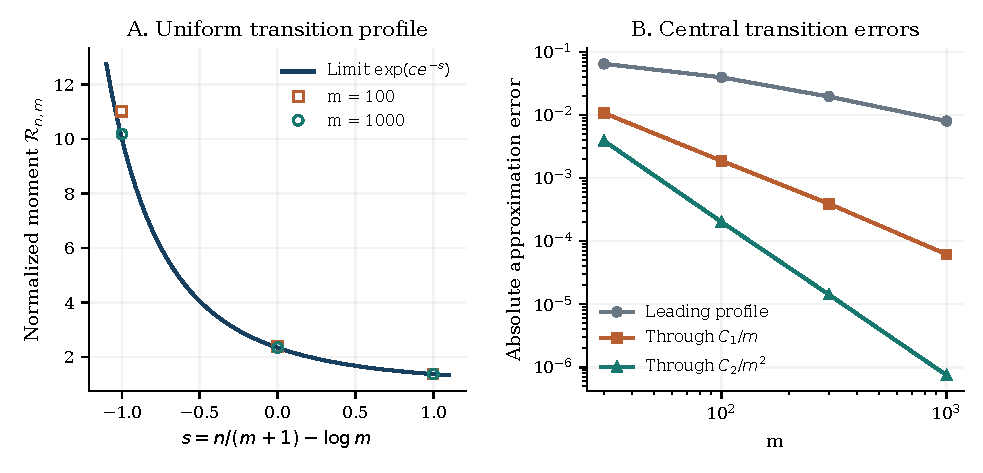
\includegraphics[width=\textwidth]{../figures/moment_transition.pdf}
\caption{The proved profile $\exp(c e^{-s})$ and numerical checks near
the central transition. The second panel shows errors of the successive
approximations along the four cases in Table~\ref{moment:tab}. The curves
visualize the theorem and its diagnostics; they supply no independent proof.}
\label{moment:fig}
\end{figure}
